\documentclass{article}

\usepackage{graphicx}
\usepackage{tikz}
\usepackage{tikzsymbols}
\usetikzlibrary{calc,patterns,shapes.geometric}
\pagestyle{empty}
\usepackage[margin=0pt]{geometry}
\geometry{papersize={14in,12in}}

\def\centerarc[#1](#2)(#3:#4:#5){\draw[#1] ($(#2)+({#5*cos(#3)},{#5*sin(#3)})$) arc (#3:#4:#5);}

\begin{document}
	\begin{figure}
		\centering
		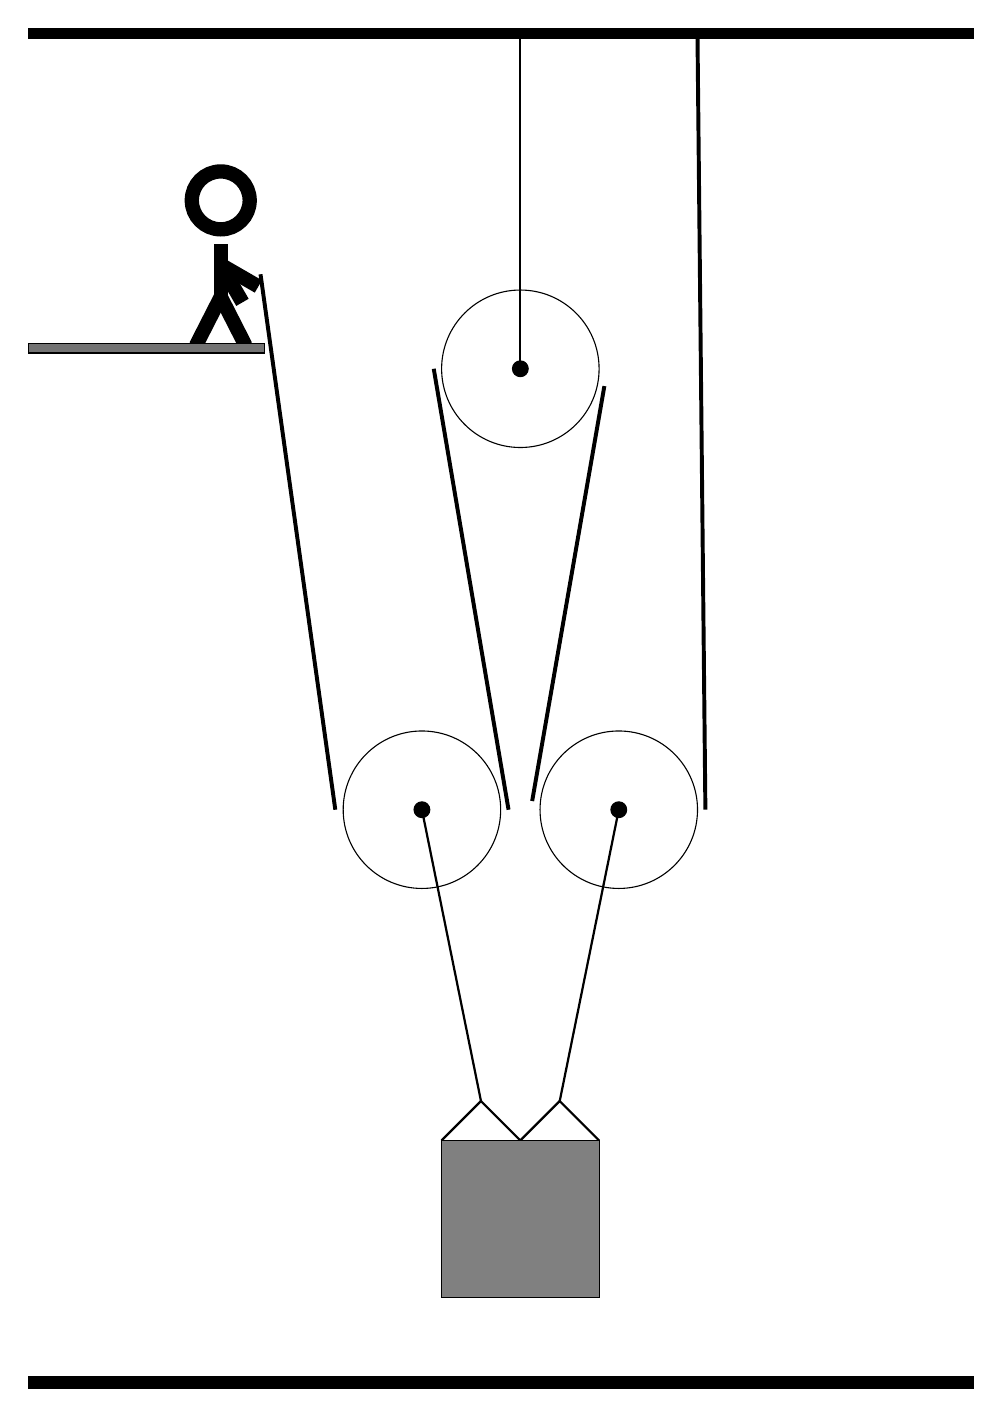
\begin{tikzpicture}
			%%%%% START %%%%%
			\draw[fill=black] (-4, 14) rectangle (8, 14.125);
			
			\draw (1, 4.2) circle (1);
			\draw[fill=black] (1, 4.2) circle (0.1);
			
			\draw (2.25, 9.8) circle (1);
			\draw[fill=black] (2.25, 9.8) circle (0.1);
			\draw[thick] (2.25, 9.8) -- (2.25, 14);
			
			\draw (3.5, 4.2) circle (1);
			\draw[fill=black] (3.5, 4.2) circle (0.1);
			
			\draw[thick] (3.5, 4.2) -- (2.75, 0.5);
			\draw[thick] (1, 4.2) -- (1.75, 0.5);
			\draw[thick]  (1.25, 0) -- (1.75, 0.5) -- (2.25, 0);
			\draw[thick]  (2.25, 0) -- (2.75, 0.5) -- (3.25, 0);
			\draw[fill=black!50] (1.25, 0) rectangle (3.25, -2);
			
			\draw[line width=0.5mm] (-1.05, 11) --  (-0.1, 4.2);
			\centerarc[line width=0.5mm](1, 4.2)(180:360:1.1);
			\draw[line width=0.5mm] (2.1, 4.2) -- (1.15, 9.8);
			\centerarc[line width=0.5mm](2.25, 9.8)(-20:180:1.1);
			\draw[line width=0.5mm](3.317, 9.58) -- (2.4, 4.31);
			\centerarc[line width=0.5mm](3.5, 4.2)(160:360:1.1);
			\draw[line width=0.5mm](4.6, 4.2) -- (4.5, 14);
			
			\node at (-1.5, 11.2) {\Strichmaxerl[10][120][-30]};
			\draw[fill=black!55] (-4, 10) rectangle (-1, 10.125);
			
			\draw[fill=black] (-4, -3) rectangle (8, -3.15);
			%%%%% END %%%%%
		\end{tikzpicture}
	\end{figure}	
\end{document}